\documentclass[10pt,aspectratio=169]{ntuabeamer}
\usepackage{appendixnumberbeamer}

\graphicspath{{assets/}}

\usepackage{tikz}
% One plain sentence closing a frame: what the audience should take away.
\newcommand{\takeaway}[1]{\par\vspace{0.7em}\textcolor{ntuablue}{\textbf{So} #1}\par}

\framesource{sandia2014}{Kalashnikova et al.\ \href{https://www.osti.gov/biblio/1177206}{\emph{Reduced Order Modeling for Prediction and Control of Large-Scale Systems}}. Sandia Report SAND2014-4693, 2014.}
\framesource{bai2021}{Bai~Z., Peng~L. \href{https://doi.org/10.1186/s40323-021-00213-5}{\emph{Non-intrusive nonlinear model reduction via machine learning approximations to low-dimensional operators}}. Adv.\ Model.\ Simul.\ Eng.\ Sci., 2021.}
\framesource{kutz2016}{Kutz, Brunton, Brunton, Proctor. \href{https://epubs.siam.org/doi/book/10.1137/1.9781611974508}{\emph{Dynamic Mode Decomposition: Data-Driven Modeling of Complex Systems}}. SIAM, 2016.}

\title{Principal Component Analysis and Reduced-Order Modeling}
\subtitle{Reduced-order modeling motivation, workflow, and principal component analysis as a concrete construction}
\author{NTUA School of Civil Engineering}
\date{\today}

\begin{document}

\begin{frame}[plain]
  \makepresentationtitle
\end{frame}

\begin{frame}{Roadmap}
  \small
  \tableofcontents

  \vspace{0.6em}
  The question that drives the deck: \emph{how can we replace an expensive simulation by a much smaller model that is almost as accurate?}
  We first see why this is useful, then how PCA finds the few shapes that matter, then how to use them inside the governing equations.
\end{frame}

\section{Why a Reduced-Order Model?}
\sectiondivider{Why a Reduced-Order Model?}

\begin{frame}{Why Reduced-Order Modeling?}
  \small
  Many tasks need the \emph{same} simulation again and again for different inputs:
  design optimization, uncertainty analysis, real-time monitoring.
  Each input is a \textcolor{ntuablue}{query}.

  \begin{itemize}
    \item \(\xi\): the parameters of one query, e.g.\ a load magnitude and a material stiffness
    \item \(\bd{u}(\xi)\): the computed state for that query, e.g.\ all nodal displacements of a finite-element model
    \item \(D\): number of numbers in \(\bd{u}\) (one per unknown), often thousands to millions; so \(\bd{u}(\xi)\in\mathbb{R}^{D}\)
  \end{itemize}

  \vspace{0.3em}
  Example: if one full solve takes 1 hour, then 10\,000 queries take more than a year.

  \takeaway{if every query needs a full solve, many-query tasks are out of reach.}
\end{frame}

\begin{frame}{The Key Observation}
  \small
  Take one structure and vary only the load magnitude \(\xi\).
  The response is linear in the load, so
  \[
    \bd{u}(\xi)=\xi\,\bd{u}(1).
  \]
  All \(D\) displacements, for every \(\xi\), are described by \emph{one} number \(\xi\) times a fixed shape.

  \vspace{0.4em}
  With several parameters, or a nonlinear response, the states are no longer on a line,
  but they still tend to lie near a thin, low-dimensional set inside \(\mathbb{R}^{D}\):
  nearby queries give similar states.

  \takeaway{we do not need all \(D\) numbers to describe every state; a handful of shapes can be enough.}
\end{frame}

\begin{frame}{What a Reduced-Order Model Does}
  \small
  A reduced-order model (ROM) describes each state by \(r\ll D\) numbers and rebuilds the full state from them:
  \[
    \bd{u}(\xi)\in\mathbb{R}^{D}
    \;\xrightarrow{\;\mathrm{Enc}_r\;}\;
    \bd{u}_r\in\mathbb{R}^{r}
    \;\xrightarrow{\;\mathrm{Dec}_r\;}\;
    \widehat{\bd{u}}(\xi)\in\mathbb{R}^{D}
  \]

  \begin{itemize}
    \item \(r\): reduced dimension, the number of numbers we keep
    \item \(\mathrm{Enc}_r\) (encoder): compresses a full state to \(r\) numbers \(\bd{u}_r\)
    \item \(\mathrm{Dec}_r\) (decoder): rebuilds an approximate full state \(\widehat{\bd{u}}\approx\bd{u}\)
  \end{itemize}

  \vspace{0.3em}
  Compression alone is not enough: for a new query we do not know \(\bd{u}\) yet.
  The ROM must therefore \emph{compute} \(\bd{u}_r\) directly, by solving a small problem in \(\mathbb{R}^{r}\).
  Methods that use the model's internal matrices to do this are called \emph{intrusive}
  (this deck); data-only variants are \emph{non-intrusive}\framecite{bai2021}.

  \takeaway{a ROM is a cheap compressor plus a cheap solver for the compressed numbers.}
\end{frame}

\begin{frame}{High-Level Workflow}
  \small
  Expensive work is done once offline on \(N_{\mathrm{train}}\) training queries;
  then \(N_{\mathrm{deploy}}\) new queries are answered online.

  \threecols
  {
    \textcolor{ntuablue}{Offline: data}
    \begin{itemize}
      \item Sample \(\xi_1,\dots,\xi_{N_{\mathrm{train}}}\)
      \item Run the full model for each
      \item Store the states \(\bd{u}(\xi_j)\in\mathbb{R}^D\) (\emph{snapshots})
    \end{itemize}
  }
  {
    \textcolor{ntuablue}{Offline: model}
    \begin{itemize}
      \item Build a reduced basis of size \(r\ll D\)
      \item Form \(\mathrm{Enc}_r,\,\mathrm{Dec}_r\)
      \item Assemble the reduced model
    \end{itemize}
  }
  {
    \textcolor{ntuablue}{Online: deploy}
    \begin{itemize}
      \item New query \(\xi_i\)
      \item Solve the small reduced model in \(\mathbb{R}^r\)
      \item Reconstruct \(\widehat{\bd{u}}(\xi_i)=\mathrm{Dec}_r(\bd{u}_r(\xi_i))\)
    \end{itemize}
  }

  \takeaway{we pay for training once, then every new query is cheap.}
\end{frame}

\begin{frame}{When Does a ROM Pay Off?\framecite{sandia2014}}
  \small
  Offline cost \(T_{\mathrm{off}}\): the \(N_{\mathrm{train}}\) full solves plus the time to build the basis.
  Each later query saves \(t_{\mathrm{HF}}-t_{\mathrm{ROM}}\), where \(t_{\mathrm{HF}}\) is the time of one full
  (high-fidelity) solve and \(t_{\mathrm{ROM}}\ll t_{\mathrm{HF}}\) the time of one ROM solve.
  The ROM wins once the number of queries \(N_{\mathrm{use}}\) satisfies
  \[
    N_{\mathrm{use}}
    >
    \frac{T_{\mathrm{off}}}
         {t_{\mathrm{HF}} - t_{\mathrm{ROM}}}.
  \]

  \textcolor{ntuablue}{Example.} \(t_{\mathrm{HF}}=1\) h, \(N_{\mathrm{train}}=100\), basis building 2 h, \(t_{\mathrm{ROM}}=1\) s:
  \(T_{\mathrm{off}}=100+2=102\) h, so \(N_{\mathrm{use}}>102\,\mathrm{h}/(1\,\mathrm{h}-1\,\mathrm{s})\approx 102\) queries.
  After the 103rd query every further query is almost free.

  \takeaway{a ROM pays off only if it will be used for many more queries than were needed to train it.}
\end{frame}

\begin{frame}{Recap: Why a ROM?}
  \small
  We learned that similar states can be described by a few numbers, so a ROM (encoder, decoder and small solver) pays off when used many times; next, principal component analysis finds those few numbers from data.
\end{frame}

\section{PCA: Finding the Important Directions}
\sectiondivider{PCA: Finding the Important Directions}

\begin{frame}{PCA Snapshot Basis\framecite{kutz2016}}
  \small
  In the ROM literature this construction is often called
  \textcolor{ntuablue}{proper orthogonal decomposition (POD)}; we use the name
  \textcolor{ntuablue}{principal component analysis (PCA)}.

  Stack the snapshots as rows, compute their mean, and subtract it:
  \[
    \bar{\bd{u}}
    =
    \frac{1}{N_{\mathrm{train}}}
    \sum_{j=1}^{N_{\mathrm{train}}}
    \bd{u}(\xi_j),
    \qquad
    \bd{U}_c
    =
    \begin{bmatrix}
      (\bd{u}(\xi_1)-\bar{\bd{u}})^{\top} \\
      \vdots \\
      (\bd{u}(\xi_{N_{\mathrm{train}}})-\bar{\bd{u}})^{\top}
    \end{bmatrix}
    \in \mathbb{R}^{N_{\mathrm{train}} \times D}
  \]

  \begin{itemize}
    \item \(\bar{\bd{u}}\in\mathbb{R}^{D}\): the mean state, the ``typical'' snapshot
    \item \(\bd{U}_c\): the \emph{centered snapshot matrix}, one row per training query
  \end{itemize}
  We subtract the mean so that what remains is only the \emph{variation} between snapshots.

  \takeaway{PCA will describe how snapshots differ from the mean, not the mean itself.}
\end{frame}

\begin{frame}{PCA Intuition}
  \begin{figure}
    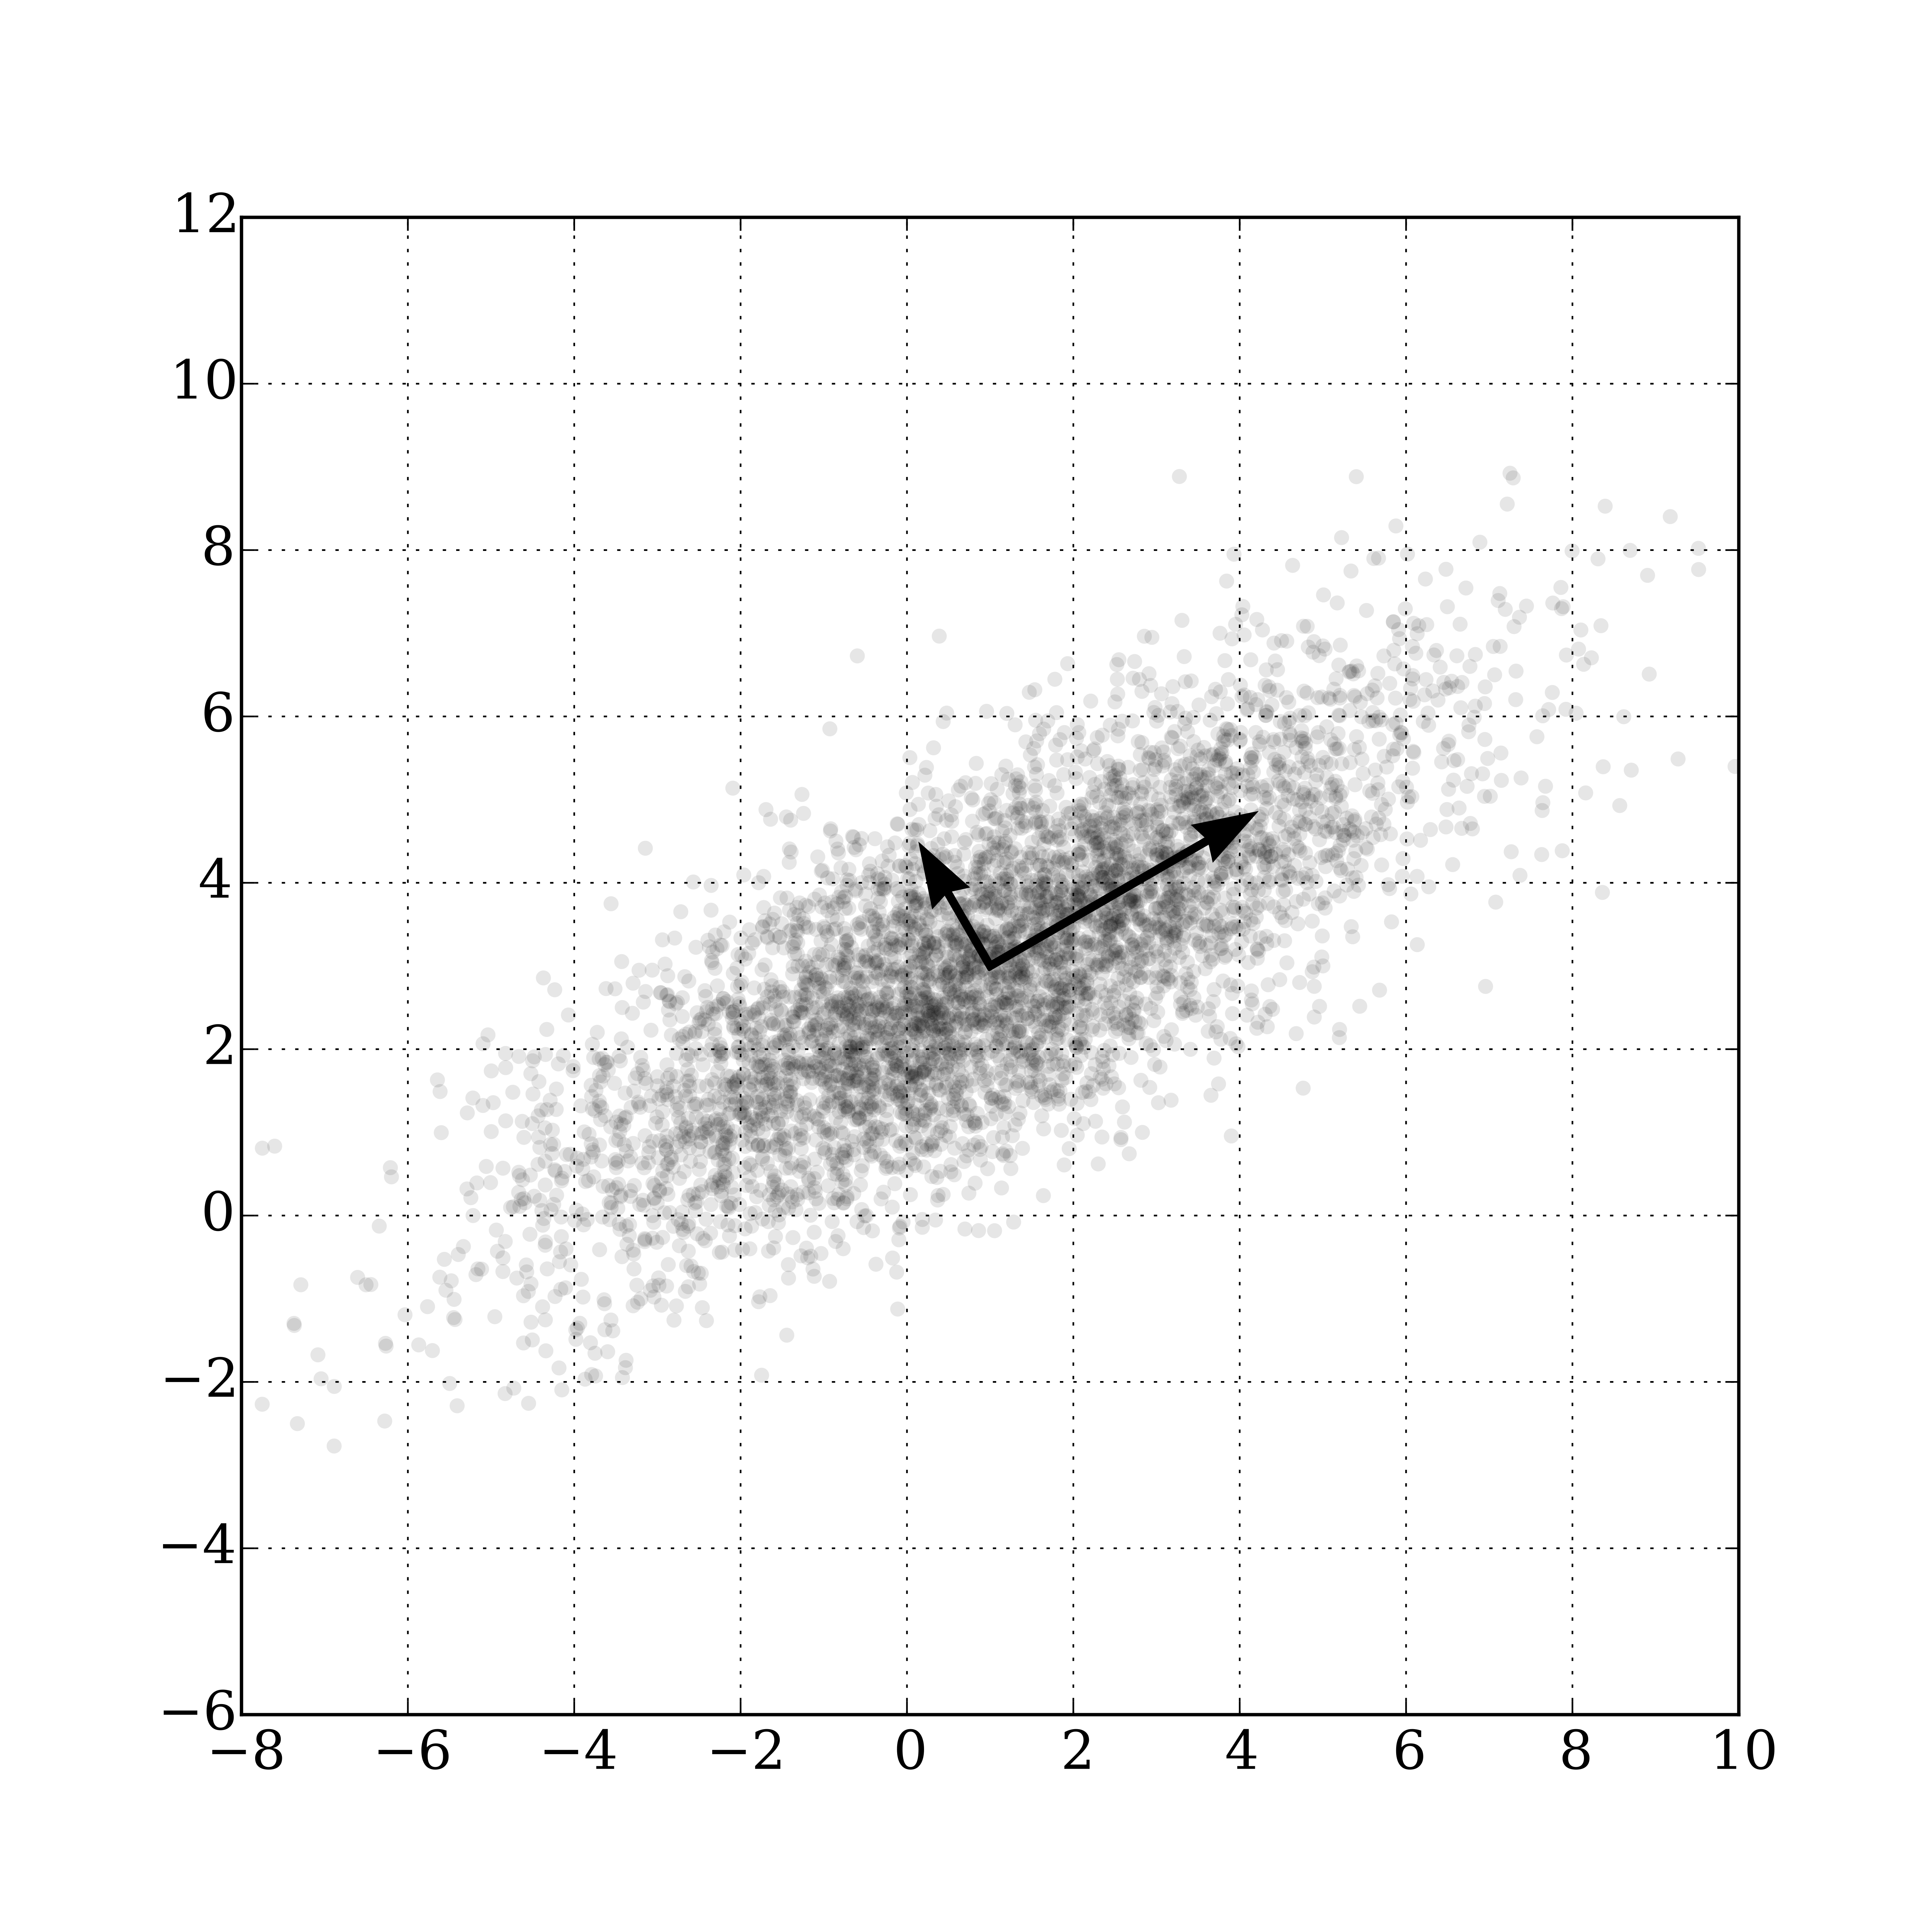
\includegraphics[width=0.85\textwidth,height=0.60\textheight,keepaspectratio]{principal-axes.png}
    \caption{\footnotesize Each snapshot \(\bd{u}(\xi_j)\) is a point in \(\mathbb{R}^D\) (drawn here for \(D=2\)).
      The arrows are the principal axes: the first points along the direction of largest spread, the second is perpendicular to it.}
  \end{figure}
  \small
  \takeaway{when the points cluster near a line or plane, a few axes describe them well.}
\end{frame}

\begin{frame}{A Tiny Worked Example: the Data}
  \small
  \twocols[0.42\textwidth][0.55\textwidth]
  {
    Four snapshots in \(\mathbb{R}^2\) (\(D=2\)):
    \[
      (1,1.2),\;(2,1.8),\;(3,3.1),\;(4,3.9)
    \]
    Mean: \(\bar{\bd{u}}=(2.5,\,2.5)\).

    \medskip
    The points lie almost on one line, so one number should be enough to place each of them.
    The first principal axis is that line's direction,
    \(\bd{v}_1\approx(0.726,\,0.688)\).
  }
  {
    \begin{center}
    \begin{tikzpicture}[x=0.62cm,y=0.62cm,>=stealth]
      \draw[->,gray] (0,0) -- (5.2,0) node[right] {\scriptsize \(u_1\)};
      \draw[->,gray] (0,0) -- (0,5.2) node[above] {\scriptsize \(u_2\)};
      \draw[ntuablue,thick] (2.5-2.7*0.726,2.5-2.7*0.688) -- (2.5+2.7*0.726,2.5+2.7*0.688)
        node[above right] {\scriptsize axis \(\bd{v}_1\)};
      \foreach \x/\y in {1/1.2,2/1.8,3/3.1,4/3.9}
        \fill[orange!85!black] (\x,\y) circle (2.5pt);
      \fill[black] (2.5,2.5) circle (2pt) node[below right] {\scriptsize mean};
    \end{tikzpicture}
    \end{center}
  }

  \takeaway{PCA finds the line through the mean along which the data vary most (in general, a subspace).}
\end{frame}

\begin{frame}{A Tiny Worked Example: Encode and Decode}
  \small
  Variance along each axis (eigenvalues of the covariance matrix, next frame):
  \(\lambda_1=2.364\) along \(\bd{v}_1\) and \(\lambda_2=0.011\) along the perpendicular axis.
  Axis 1 carries \(2.364/(2.364+0.011)\approx 99.5\%\) of the variance, so keep \(r=1\).

  \medskip
  Take the snapshot \(\bd{u}=(1,\,1.2)\):
  \begin{align*}
    \text{encode: } & u_r=\bd{v}_1^{\top}(\bd{u}-\bar{\bd{u}})
      = 0.726\cdot(-1.5)+0.688\cdot(-1.3)\approx -1.98
      && \text{(one number)}\\
    \text{decode: } & \widehat{\bd{u}}=\bar{\bd{u}}+u_r\bd{v}_1\approx(1.06,\,1.14)
      && \text{(back in } \mathbb{R}^2\text{)}
  \end{align*}
  The error is \(\|\widehat{\bd{u}}-\bd{u}\|\approx 0.09\), small compared with the data spread (about 4).

  \takeaway{one number per snapshot reproduces the data to within a few percent, because the discarded axis carries only 0.5\% of the variance.}
\end{frame}

\begin{frame}{PCA Basis Construction}
  \small
  The principal axes are found from the \emph{covariance matrix}, which records how the state entries vary together over the snapshots:
  \[
    \bd{C}=\frac{1}{N_{\mathrm{train}}}\bd{U}_c^{\top}\bd{U}_c\in\mathbb{R}^{D\times D},
    \qquad
    \bd{C}\bd{v}_i=\lambda_i\bd{v}_i .
  \]
  The second equation says: \(\bd{v}_i\) is an \emph{eigenvector} of \(\bd{C}\) (a direction that \(\bd{C}\) only stretches)
  and \(\lambda_i\) the \emph{eigenvalue} (the stretch factor).

  \begin{itemize}
    \item \(\bd{v}_i\): principal axis \(i\); the axes are perpendicular to each other and ordered by \(\lambda_i\)
    \item \(\lambda_i\): the variance of the snapshots along \(\bd{v}_i\); large \(\lambda_i\) means an important direction
  \end{itemize}
  Why the eigenvectors are the right directions: see the appendix.

  \takeaway{PCA reduces to one standard computation: the eigenvectors of \(\bd{C}\) with the largest eigenvalues.}
\end{frame}

\begin{frame}{PCA Encoder and Decoder}
  \small
  Keep the first \(r\) axes as columns,
  \(\bd{V}_r=[\bd{v}_1,\dots,\bd{v}_r]\in\mathbb{R}^{D\times r}\). Then:

  \begin{itemize}
    \item \(\mathrm{Enc}_r\): \(\bd{u}_r=\bd{V}_r^{\top}(\bd{u}-\bar{\bd{u}})\)
          \quad each entry is the coordinate of \(\bd{u}-\bar{\bd{u}}\) along one kept axis
    \item \(\mathrm{Dec}_r\): \(\widehat{\bd{u}}=\bar{\bd{u}}+\bd{V}_r\bd{u}_r\)
          \quad the mean plus a combination of the kept axes, weighted by \(\bd{u}_r\)
  \end{itemize}

  This is exactly the computation of the tiny example, with \(\bd{V}_1=\bd{v}_1\).
  The decoder is linear and independent of \(\xi\); that is what makes the later reduced equations small.

  \takeaway{PCA gives a linear encoder and decoder built from the \(r\) most important variation directions.}
\end{frame}

\begin{frame}{Eigenvalue Decay}
  \small
  Order the eigenvalues \(\lambda_1\geq\lambda_2\geq\cdots\geq 0\).
  Each \(\lambda_i\) is the variance carried by mode \(i\).

  \begin{figure}
    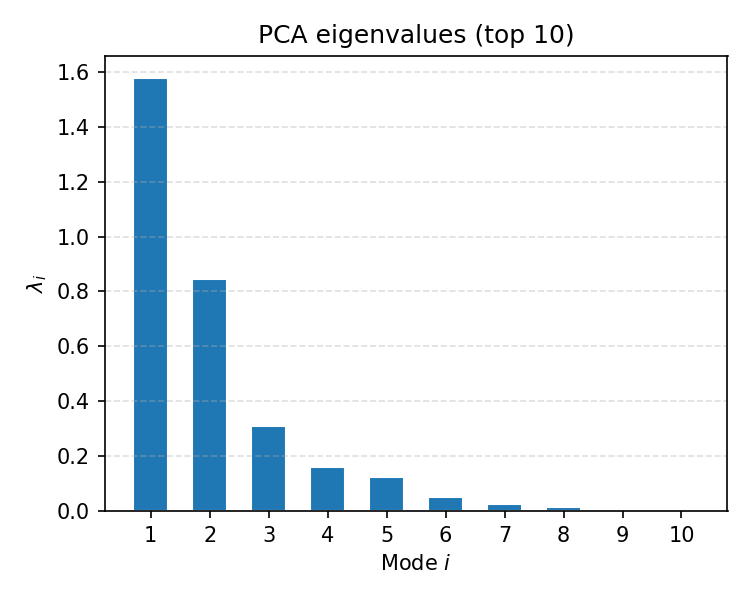
\includegraphics[width=\textwidth,height=0.50\textheight,keepaspectratio]{eigenvalues.png}
    \caption{\footnotesize Leading PCA eigenvalues. \emph{A different dataset from the worked example:}
      \(D=30\) snapshots of a Gaussian bump with random center and width, \(N_{\mathrm{train}}=200\).}
  \end{figure}
  \takeaway{when the eigenvalues fall quickly, a few modes suffice; a slow decay means the ROM needs a large \(r\).}
\end{frame}

\begin{frame}{Choosing the Reduced Dimension \(r\)}
  \small
  \twocols[0.45\textwidth][0.51\textwidth]
  {
    The \textcolor{ntuablue}{cumulative explained variance}
    \[
      \eta(r)
      =
      \frac{\sum_{i=1}^{r} \lambda_i}
           {\sum_{i=1}^{D} \lambda_i}
    \]
    is the fraction of the total variance kept by the first \(r\) modes.

    \begin{itemize}
      \item Choose the smallest \(r\) with \(\eta(r)\) above a target, e.g.\ 95\%
      \item \(1-\eta(r)\) is the variance thrown away
    \end{itemize}
  }
  {
    \begin{figure}
      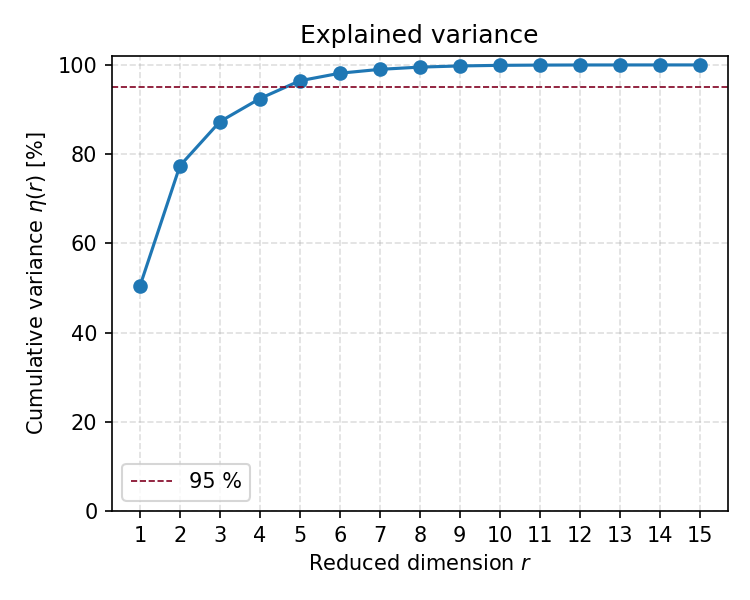
\includegraphics[width=\textwidth,height=0.52\textheight,keepaspectratio]{explained-variance.png}
      \caption{\footnotesize Same \(D=30\) Gaussian-bump dataset as the eigenvalue figure: 95\% is reached at \(r=5\).}
    \end{figure}
  }
  \takeaway{here 5 modes instead of 30 numbers keep 95\% of the variance; the target sets the accuracy.}
\end{frame}

\begin{frame}{Recap: PCA}
  \small
  We learned that PCA turns snapshots into a mean and ordered axes whose first $r$ give an encoder, a decoder and a rule for choosing $r$; next we put this basis into the equation \(\bd{K}\bd{u}=\bd{f}\) so new queries are solved with $r$ unknowns.
\end{frame}

\section{Using PCA Inside the Equations}
\sectiondivider{Using PCA Inside the Equations}

\begin{frame}{Why We Need More Than Compression}
  \small
  Encoding a state needs the state: \(\bd{u}_r=\bd{V}_r^{\top}(\bd{u}-\bar{\bd{u}})\).
  For a new query \(\xi\) we do not have \(\bd{u}(\xi)\) (that is what the full solve would give).
  We need an equation that tells us \(\bd{u}_r\) directly.

  \vspace{0.3em}
  The equation comes from the physics. For a linear structural model it reads
  \[
    \bd{K}(\xi)\,\bd{u}(\xi) = \bd{f}(\xi),
  \]
  with \(\bd{K}\in\mathbb{R}^{D\times D}\) the \emph{stiffness matrix} (how strongly the structure resists being displaced),
  \(\bd{f}\) the load vector, and \(\bd{u}\) the displacements. For a single spring this is \(k\,u=f\): stiffness times displacement equals force.

  \takeaway{we will insert the PCA decoder into \(\bd{K}\bd{u}=\bd{f}\) to get an equation for the \(r\) numbers \(\bd{u}_r\).}
\end{frame}

\begin{frame}{PCA-ROM: Substituting the Basis}
  \small
  Replace \(\bd{u}\) by the decoder \(\bar{\bd{u}}+\bd{V}_r\bd{u}_r\) and move the known mean to the right:
  \[
    \bd{K}(\xi)\bigl(\bar{\bd{u}}+\bd{V}_r\bd{u}_r\bigr)=\bd{f}(\xi)
    \quad\Longrightarrow\quad
    \bd{K}(\xi)\bd{V}_r\,\bd{u}_r
    =
    \underbrace{\bd{f}(\xi)-\bd{K}(\xi)\bar{\bd{u}}}_{\text{load not yet explained by the mean}} .
  \]
  Count: \(D\) equations, but only \(r\) unknowns in \(\bd{u}_r\).
  Because \(r<D\), we cannot satisfy all \(D\) equations exactly. Usually no \(\bd{u}_r\) makes the leftover error, the
  \emph{residual}
  \[
    \bd{r}=\bd{K}(\xi)\bd{V}_r\bd{u}_r-\bigl(\bd{f}(\xi)-\bd{K}(\xi)\bar{\bd{u}}\bigr)\in\mathbb{R}^{D},
  \]
  equal to zero.

  \takeaway{we must choose which \(r\) combinations of the equations to enforce; the Galerkin projection is the standard choice.}
\end{frame}

\begin{frame}{Galerkin: Make the Residual Invisible to the Basis}
  \small
  \twocols[0.50\textwidth][0.46\textwidth]
  {
    \textcolor{ntuablue}{Galerkin} means: pick \(\bd{u}_r\) so that the residual is perpendicular to every kept axis,
    \[
      \bd{V}_r^{\top}\bd{r}=\bd{0}.
    \]
    This is \(r\) equations for \(r\) unknowns, so a solution exists (for the usual stiffness matrices).

    \medskip
    In words: whatever error is left lies \emph{outside} the space spanned by the basis, so the reduced model cannot detect it and has no further reason to change \(\bd{u}_r\).
  }
  {
    \begin{center}
    \begin{tikzpicture}[>=stealth]
      \fill[ntuablue!10] (-2.2,-0.9) -- (2.2,-0.9) -- (2.6,0.5) -- (-1.8,0.5) -- cycle;
      \node[ntuablue] at (0.2,-0.4) {\scriptsize span of kept axes};
      \draw[->,thick,red!70!black] (0.4,-0.2) -- (0.4,1.9) node[right] {\scriptsize residual \(\bd{r}\)};
      \draw (0.4,-0.2) ++(0.25,0) -- ++(0,0.25) -- ++(-0.25,0);
    \end{tikzpicture}
    \end{center}
  }

  \takeaway{Galerkin chooses the reduced solution whose leftover error is perpendicular to the space the model can represent.}
\end{frame}

\begin{frame}{PCA-ROM: The Reduced System}
  \small
  Writing \(\bd{V}_r^{\top}\bd{r}=\bd{0}\) out gives a small \(r\times r\) system:
  \[
    \bd{K}_r(\xi)\,\bd{u}_r(\xi) = \bd{f}_r(\xi),
    \qquad
    \bd{K}_r=\bd{V}_r^{\top}\bd{K}(\xi)\bd{V}_r\in\mathbb{R}^{r\times r},
    \quad
    \bd{f}_r=\bd{V}_r^{\top}\!\bigl(\bd{f}(\xi)-\bd{K}(\xi)\bar{\bd{u}}\bigr)\in\mathbb{R}^{r}.
  \]
  Then decode: \(\widehat{\bd{u}}(\xi)=\bar{\bd{u}}+\bd{V}_r\bd{u}_r(\xi)\).

  \begin{itemize}
    \item \textcolor{ntuablue}{Offline:} full solves, mean \(\bar{\bd{u}}\), PCA basis \(\bd{V}_r\)
    \item \textcolor{ntuablue}{Online, per query:} form \(\bd{K}_r,\bd{f}_r\), solve the \(r\times r\) system, decode
  \end{itemize}
  The term \(-\bd{K}\bar{\bd{u}}\) in \(\bd{f}_r\) is essential: it accounts for the mean we subtracted (see the error frame below).

  \takeaway{one \(D\times D\) problem becomes one \(r\times r\) problem, with a decoder to return to the full state.}
\end{frame}

\begin{frame}{Worked Example: the Snapshot Cloud}
  \small
  A deliberately tiny model: \(D=3\), \(r=2\), \(N_{\mathrm{train}}=N_{\mathrm{deploy}}=200\),
  \(\xi=(\xi_1,\xi_2)\sim\mathrm{Uniform}([0,3]\times[0,2])\), with a tridiagonal \(\bd{K}(\xi_1)\) and a load \(\bd{f}(\xi_1,\xi_2)\).
  Here \(r\ll D\) does \emph{not} hold: \(D=3\) is chosen only so the cloud can be drawn.

  \begin{figure}
    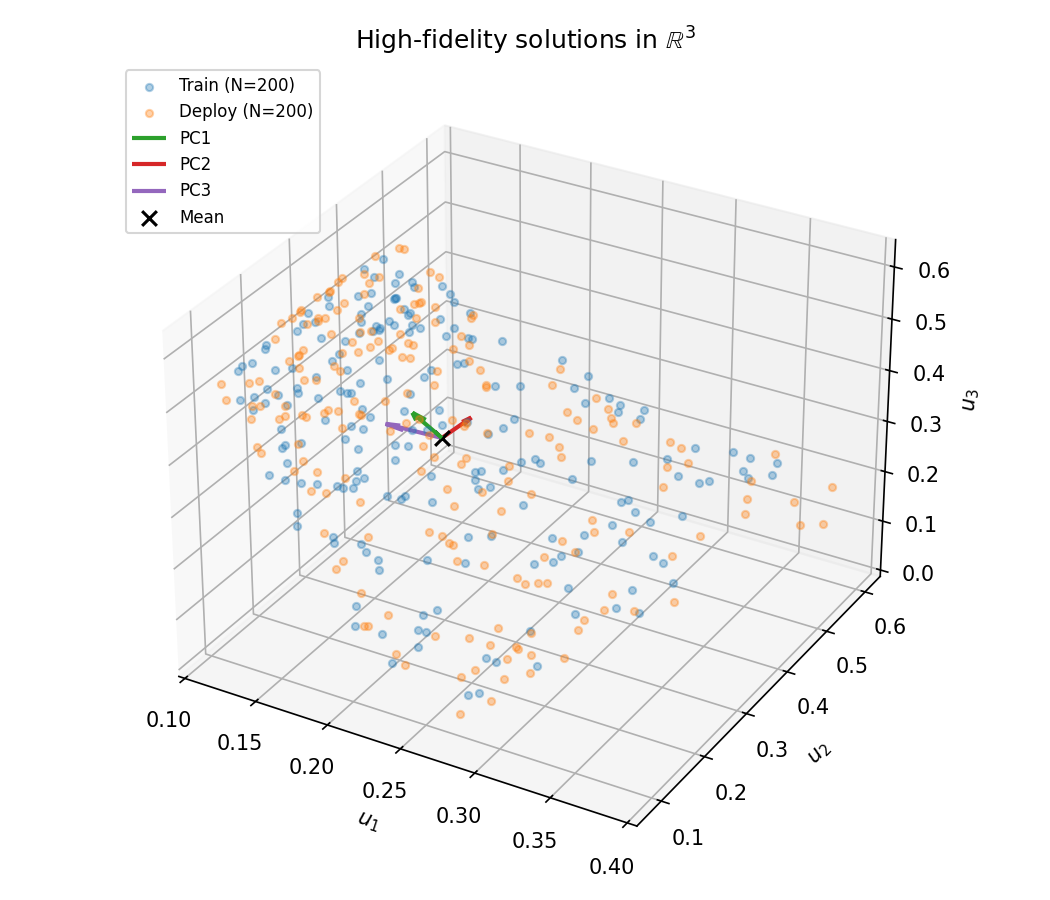
\includegraphics[width=\textwidth,height=0.48\textheight,keepaspectratio]{3d-original-space.png}
    \caption{\footnotesize All snapshots in \(\mathbb{R}^3\)
      (\textcolor{ntuablue}{blue}: train, \textcolor{orange}{orange}: deploy). Arrows: principal axes from \(\bar{\bd{u}}\).}
  \end{figure}
  \takeaway{the cloud is nearly flat, so a 2-D plane (\(r=2\)) already holds most of it; the third axis is short.}
\end{frame}

\begin{frame}{Worked Example: the Encoded Snapshots}
  \small
  \twocols[0.48\textwidth][0.48\textwidth]
  {
    The encoder \(\bd{u}_r=\bd{V}_r^{\top}(\bd{u}-\bar{\bd{u}})\) maps each snapshot to two numbers.

    \medskip
    Deployment points (orange) fall in the same region as the training points (blue): the basis learned from training queries also describes new queries.

    \medskip
    The origin is the mean state \(\bar{\bd{u}}\).
  }
  {
    \begin{figure}
      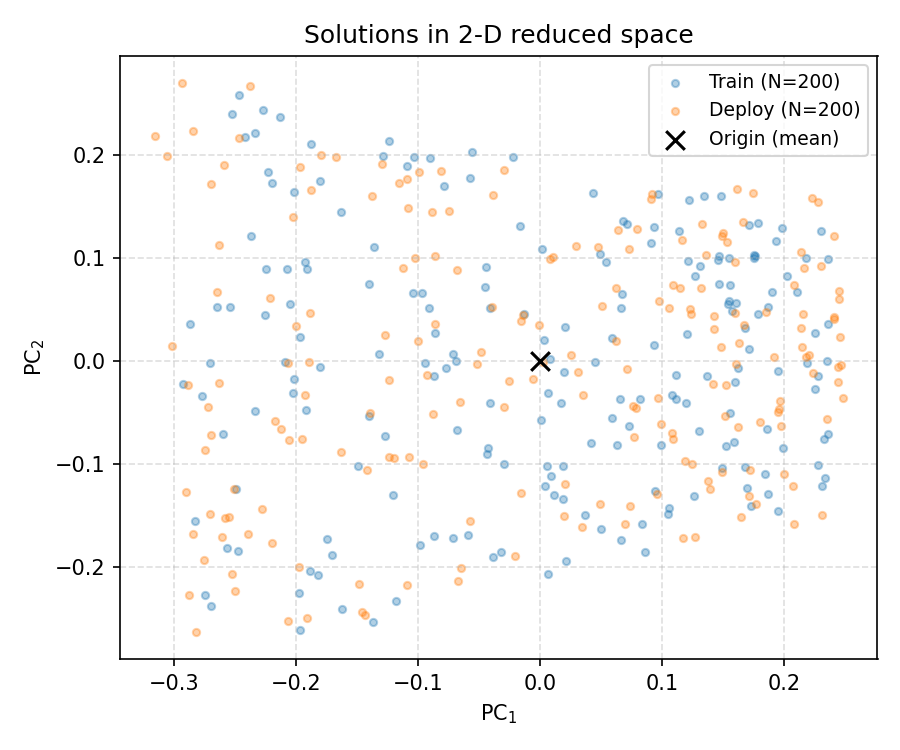
\includegraphics[width=\textwidth,height=0.62\textheight,keepaspectratio]{2d-reduced-space.png}
      \caption{\footnotesize The same snapshots encoded to \(\mathbb{R}^2\).}
    \end{figure}
  }
  \takeaway{two numbers per query describe the state; the training basis generalizes to unseen queries here.}
\end{frame}

\begin{frame}{Worked Example: One Query in Numbers}
  \small
  Query \(\xi=(1.5,\,1)\), basis from the 200 training snapshots (seed 42):
  \[
    \bd{K}=\begin{bmatrix}7&-1&0\\-1&5.5&-1\\0&-1&4.75\end{bmatrix}\!,\quad
    \bd{f}=\begin{bmatrix}1\\1\\1.5\end{bmatrix}
    \;\Longrightarrow\;
    \bd{K}_r\approx\begin{bmatrix}5.31&-0.69\\-0.69&4.68\end{bmatrix}\!,\quad
    \bd{f}_r\approx\begin{bmatrix}0.149\\-0.043\end{bmatrix}.
  \]
  Solving the \(2\times2\) system and decoding:
  \[
    \bd{u}_r\approx\begin{bmatrix}0.0274\\-0.0052\end{bmatrix}
    \;\Longrightarrow\;
    \widehat{\bd{u}}\approx(0.191,\,0.283,\,0.379)
    \quad\text{vs.}\quad
    \bd{u}=(0.183,\,0.283,\,0.376).
  \]
  Relative error: \(\|\widehat{\bd{u}}-\bd{u}\|/\|\bd{u}\|\approx 1.6\%\).
  (The signs in \(\bd{K}_r,\bd{f}_r\) depend on the arbitrary sign of the eigenvectors; \(\widehat{\bd{u}}\) does not.)

  \takeaway{a \(3\times3\) solve was replaced by a \(2\times2\) solve at a cost of about 1.6\% error.}
\end{frame}

\begin{frame}{Worked Example: How Accurate Is the ROM?}
  \small
  \twocols[0.40\textwidth][0.57\textwidth]
  {
    Relative error \(\|\widehat{\bd{u}}-\bd{u}\|/\|\bd{u}\|\) over all queries (seed 42):

    \begin{itemize}
      \item Two kept modes carry 99.8\% of the variance; the dropped third mode sets the error floor.
      \item ROM on deployment queries: mean 1.6\%, max 6.2\%.
      \item Plain PCA encode/decode (no equation solved): mean 1.4\%, so the Galerkin step adds almost no error.
      \item Omitting \(-\bd{K}\bar{\bd{u}}\) in \(\bd{f}_r\): mean error 78\%.
    \end{itemize}
  }
  {
    \begin{figure}
      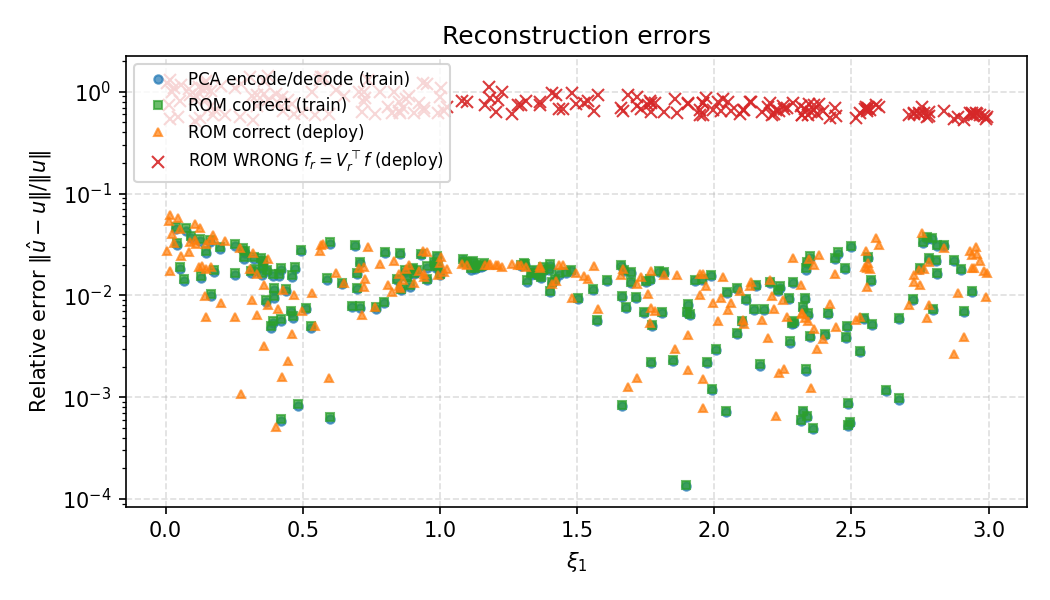
\includegraphics[width=\textwidth,height=0.48\textheight,keepaspectratio]{reconstruction-error.png}
      \caption{\footnotesize Relative error versus \(\xi_1\) (log scale). The error is small but not zero: it is the price of keeping \(r=2\) of \(D=3\) modes.}
    \end{figure}
  }
  \takeaway{the ROM is accurate to a few percent, limited by truncation, if the mean term is included.}
\end{frame}

\begin{frame}{Recap: PCA-Galerkin ROM}
  \small
  We learned that substituting the decoder and demanding a residual perpendicular to the basis gives an \(r\times r\) system (in the example, \(3\times3\) became \(2\times2\) at about 1.6\% error); the appendix collects the linear algebra behind PCA.
\end{frame}

\appendix
\sectiondivider{Appendix: optional depth}

\begin{frame}{Appendix: Why the Eigenvectors of \(\bd{C}\)?}
  \small
  The first axis is the unit direction with the largest variance of the projected snapshots.
  Since \(\bd{U}_c\) is centered, that variance is
  \[
    \max_{\|\bd{v}\|=1}\;\mathrm{Var}(\bd{U}_c\bd{v})
    =
    \max_{\|\bd{v}\|=1}\;\bd{v}^{\top}\bd{C}\bd{v}.
  \]
  A Lagrange multiplier \(\lambda\) for the constraint \(\|\bd{v}\|^2=1\) gives the stationarity condition
  \(\bd{C}\bd{v}=\lambda\bd{v}\), and then \(\bd{v}^{\top}\bd{C}\bd{v}=\lambda\).
  So the maximizer is the eigenvector with the largest eigenvalue; \(\lambda_1\) is the variance it captures.
  Repeating in the orthogonal complement yields \(\bd{v}_2,\bd{v}_3,\dots\)

  \vspace{0.4em}
  \(\bd{C}\) is symmetric positive semidefinite, so its eigenvalues are real and nonnegative and its eigenvectors can be chosen orthonormal.
\end{frame}

\begin{frame}{Appendix: PCA via Covariance or SVD}
  \small
  Starting from the centered snapshot matrix
  \[
    \bd{U}_c \in \mathbb{R}^{N_{\mathrm{train}} \times D},
    \qquad
    \bd{C} = \frac{1}{N_{\mathrm{train}}}\bd{U}_c^{\top}\bd{U}_c \in \mathbb{R}^{D\times D},
  \]
  the PCA eigenproblem is
  \[
    \bd{C}\bd{v}_i = \lambda_i \bd{v}_i.
  \]

  The singular value decomposition (SVD) of the same matrix is
  \[
    \bd{U}_c = \bd{W}\bd{\Sigma}\bd{V}^{\top}.
  \]

  \begin{itemize}
    \item \(\bd{W} \in \mathbb{R}^{N_{\mathrm{train}} \times N_{\mathrm{train}}}\): left singular vectors, acting on the sample side
    \item \(\bd{\Sigma} \in \mathbb{R}^{N_{\mathrm{train}} \times D}\): rectangular diagonal matrix, \(\Sigma_{ii}=\sigma_i\) (the \emph{singular values})
    \item \(\bd{V} \in \mathbb{R}^{D \times D}\): right singular vectors, acting on the state/feature side
  \end{itemize}

  \textcolor{gray}{\footnotesize In practice the economy (thin) SVD is used:
    \(\bd{W}\in\mathbb{R}^{N_{\mathrm{train}}\times k}\),
    \(\bd{\Sigma}\in\mathbb{R}^{k\times k}\),
    \(k=\min(N_{\mathrm{train}},D)\).}

  Therefore (\(\bd{\Sigma}^{\top}\bd{\Sigma}=\mathrm{diag}(\sigma_i^2)\in\mathbb{R}^{D\times D}\)):
  \[
    \bd{U}_c^{\top}\bd{U}_c = \bd{V}\,\bd{\Sigma}^{\top}\bd{\Sigma}\,\bd{V}^{\top},
  \]
  so the PCA eigenvectors are the right singular vectors:
  \(\bd{v}_i = \text{column } i \text{ of } \bd{V}.\)
\end{frame}

\begin{frame}{Appendix: Relationship Between Eigenvalues}
  \small
  Since
  \[
    \bd{C} = \frac{1}{N_{\mathrm{train}}}\bd{U}_c^{\top}\bd{U}_c
    = \frac{1}{N_{\mathrm{train}}}\bd{V}\,\bd{\Sigma}^{\top}\bd{\Sigma}\,\bd{V}^{\top},
  \]
  the PCA eigenvalues and SVD singular values satisfy
  \[
    \lambda_i = \frac{\sigma_i^2}{N_{\mathrm{train}}}.
  \]

  If we instead diagonalize the smaller Gram matrix,
  \[
    \bd{G} = \frac{1}{N_{\mathrm{train}}}\bd{U}_c\bd{U}_c^{\top}
    = \frac{1}{N_{\mathrm{train}}}\bd{W}\,\bd{\Sigma}\bd{\Sigma}^{\top}\,\bd{W}^{\top},
  \]
  where \(\bd{G}\) is the sample-side Gram matrix.
  \begin{itemize}
    \item eigenvectors of \(\bd{C}\): right singular vectors \(\bd{V}\)
    \item eigenvectors of \(\bd{G}\): left singular vectors \(\bd{W}\)
    \item same nonzero eigenvalues: \(\lambda_i = \sigma_i^2/N_{\mathrm{train}}\)
    \item if \(N_{\mathrm{train}} \ll D\), solve the sample-side problem
  \end{itemize}
\end{frame}

\begin{frame}{Appendix: Explained Variance Variants}
  \small
  In terms of singular values, the cumulative explained variance is
  \[
    \eta(r) = \frac{\sum_{i=1}^{r}\sigma_i^2}{\sum_{i=1}^{D}\sigma_i^2},
  \]
  because \(\lambda_i=\sigma_i^2/N_{\mathrm{train}}\) and the factor cancels.

  \vspace{0.4em}
  The denominator is the \textbf{total variance}
  \(\sum_{i=1}^{D}\lambda_i = \mathrm{tr}(\bd{C})\),
  available directly from the diagonal of \(\bd{C}\): no full eigendecomposition is needed to evaluate it.
  At most \(\min(N_{\mathrm{train}}-1,D)\) eigenvalues are nonzero.
\end{frame}

\end{document}
